\section{Resultat}

\import{Tabeller}{all}

\subsection{Inklinasjon}

\import{Tabeller}{inklinasjon}

\begin{figure}
    \centering
    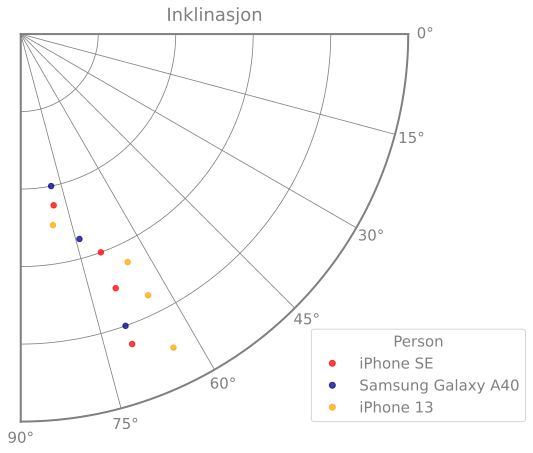
\includegraphics[width=0.75\textwidth]{Plots/inclination.png}
    \caption{Plott av inklinasjon for de forskjellige målesettene. Fargen angir hvilken telefon som ble benyttet.}
    
    \label{fig:plot_inklination}
\end{figure}


\subsection{Deklinasjon}

\import{Tabeller}{deklinasjon}

\begin{figure}
    \centering
    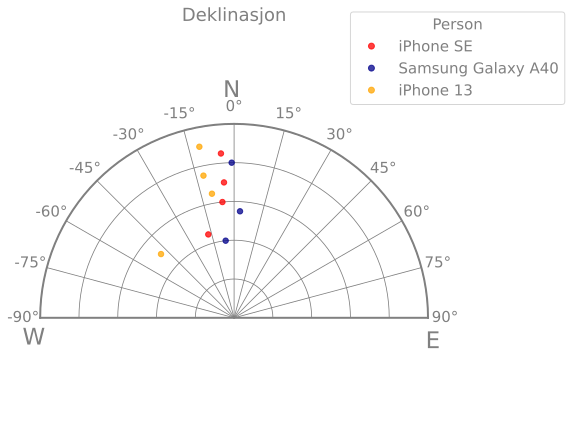
\includegraphics[width=0.75\textwidth]{Plots/declination.png}
    \caption{Plott av deklinasjon for de ulike målesettene. Fargen angir hvilken telefon som ble benyttet.}
    \label{fig:plot_declination}
\end{figure}


\begin{figure}
    \centering
    \includegraphics{img/WMM.png}
    \caption{Magnetisk deklinasjon og inklinasjon ifølge \href{https://www.magnetic-declination.com/}{magnetic-declination.com}. Denne nettsiden bruker World Magnetic Model 2020.}
    \label{fig:WMM}
\end{figure}